% How a DID and its first record are derived: operations in boxes, the
% values they pass on the arrows.
\documentclass[border=12pt]{standalone}
% The look shared by the figures drawn with TikZ: the font and the colours
% of the Mermaid diagrams (mermaid.json). Built with xelatex, see AGENTS.md.
\usepackage[no-math]{fontspec}
\setmainfont{Lato}
\setsansfont{Lato}
\renewcommand{\familydefault}{\sfdefault}
\usepackage{amsmath}
\usepackage{tikz}
\usetikzlibrary{arrows.meta,positioning,calc,fit,backgrounds}

\definecolor{navy}{HTML}{1F3A5F}
\definecolor{ink}{HTML}{1F2A37}
\definecolor{muted}{HTML}{5C6B7E}
\definecolor{blueFill}{HTML}{EEF4FB}
\definecolor{blueLine}{HTML}{5B7FAE}
\definecolor{greenFill}{HTML}{E3F4E8}
\definecolor{greenLine}{HTML}{2F8F4E}
\definecolor{amberFill}{HTML}{FDF1DC}
\definecolor{amberLine}{HTML}{C98A1B}
\definecolor{violetFill}{HTML}{F3EFFC}
\definecolor{violetLine}{HTML}{7B61B8}
\definecolor{greyFill}{HTML}{F6F8FB}
\definecolor{greyLine}{HTML}{C3CCD7}

\tikzset{
  every picture/.style={font=\small, color=ink, line cap=round},
  base/.style={rounded corners=3pt, line width=0.7pt, align=center, inner sep=5pt},
  plain/.style={base, draw=greyLine, fill=white},
  public/.style={base, draw=blueLine, fill=blueFill},
  secret/.style={base, draw=violetLine, fill=violetFill},
  result/.style={base, draw=greenLine, fill=greenFill},
  carried/.style={base, draw=amberLine, fill=amberFill},
  strong/.style={base, draw=navy, fill=navy, text=white, font=\small\bfseries},
  op/.style={base, draw=navy, fill=white, line width=0.9pt, font=\small\bfseries},
  flow/.style={-{Stealth[length=2.2mm]}, draw=muted, line width=0.7pt},
  link/.style={draw=muted, line width=0.7pt},
  data/.style={font=\footnotesize, fill=white, inner sep=1.5pt, text=ink},
}

\begin{document}
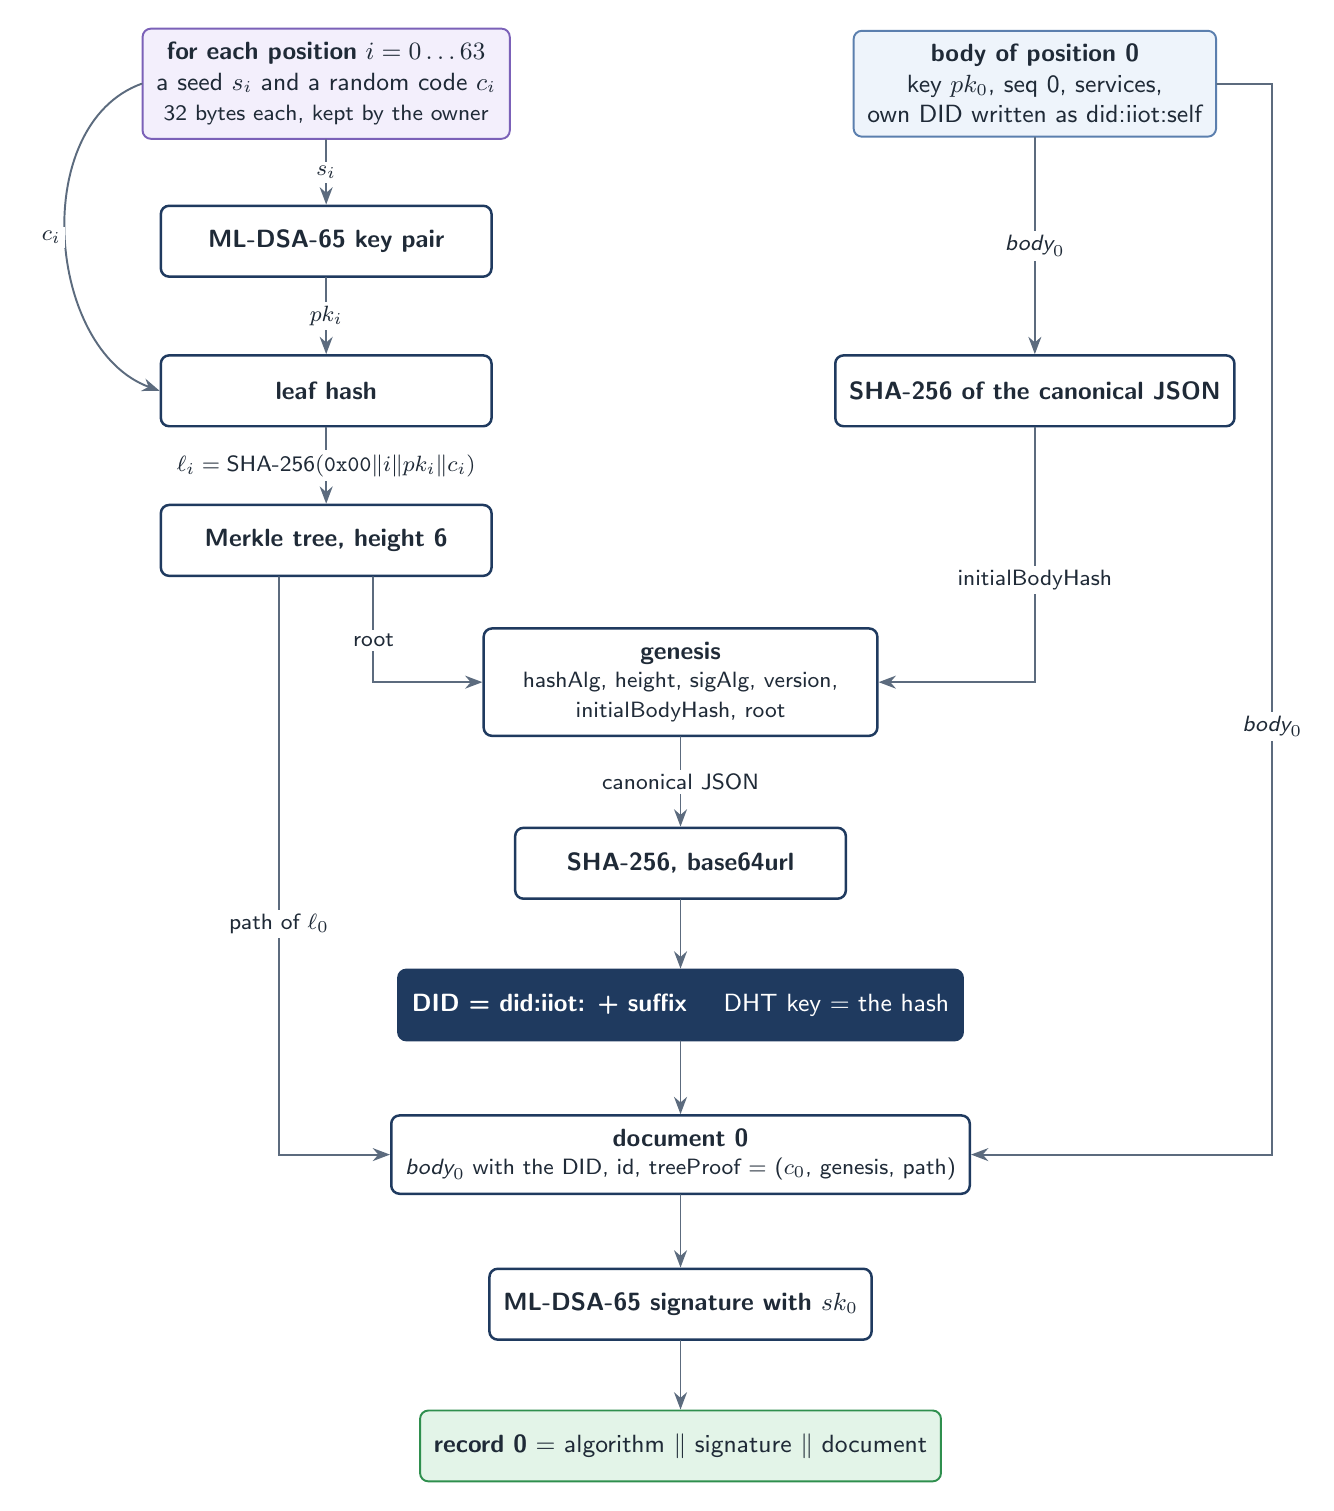
\begin{tikzpicture}[
  op/.append style={minimum width=4.2cm, minimum height=9mm},
  lbl/.style={data, pos=0.5},
]
  % inputs
  \node[secret, minimum width=4.2cm] (seeds) at (0,0)
    {\textbf{for each position} $i = 0 \ldots 63$\\ a seed $s_i$ and a random code $c_i$\\ {\footnotesize 32 bytes each, kept by the owner}};
  \node[public, minimum width=4.6cm] (body) at (9,0)
    {\textbf{body of position 0}\\ key $pk_0$, seq 0, services,\\ own DID written as did:iiot:self};

  % left column: the tree
  \node[op] (keygen) at (0,-2.0) {ML-DSA-65 key pair};
  \node[op] (leaf)   at (0,-3.9) {leaf hash};
  \node[op] (merkle) at (0,-5.8) {Merkle tree, height 6};
  \draw[flow] (seeds) -- node[lbl] {$s_i$} (keygen);
  \draw[flow] (keygen) -- node[lbl] {$pk_i$} (leaf);
  \draw[flow] (seeds.west) to[out=200, in=160] node[data, left] {$c_i$} (leaf.west);
  \draw[flow] (leaf) -- node[lbl] {$\ell_i = \text{SHA-256}(\texttt{0x00} \Vert i \Vert pk_i \Vert c_i)$} (merkle);

  % right column: the hashed body
  \node[op, minimum width=4.6cm] (bodyhash) at (9,-3.9) {SHA-256 of the canonical JSON};
  \draw[flow] (body) -- node[lbl] {$\textit{body}_0$} (bodyhash);

  % centre: genesis, DID, document, record
  \node[op, minimum width=5.0cm] (genesis) at (4.5,-7.6)
    {genesis\\[-1pt] {\footnotesize\normalfont hashAlg, height, sigAlg, version,}\\ {\footnotesize\normalfont initialBodyHash, root}};
  \node[op] (didhash) at (4.5,-9.9) {SHA-256, base64url};
  \node[strong, minimum width=5.6cm, minimum height=9mm] (did) at (4.5,-11.7)
    {DID = did:iiot: + suffix \quad{\normalfont DHT key = the hash}};
  \node[op, minimum width=5.6cm] (doc) at (4.5,-13.6)
    {document 0\\[-1pt] {\footnotesize\normalfont $\textit{body}_0$ with the DID, id, treeProof = ($c_0$, genesis, path)}};
  \node[op] (sign) at (4.5,-15.5) {ML-DSA-65 signature with $sk_0$};
  \node[result, minimum width=5.6cm, minimum height=9mm] (rec) at (4.5,-17.3)
    {\textbf{record 0} = algorithm $\Vert$ signature $\Vert$ document};

  \draw[flow] ([xshift=6mm]merkle.south) |- node[data, pos=0.3] {root} (genesis.west);
  \draw[flow] (bodyhash.south) |- node[data, pos=0.3] {initialBodyHash} (genesis.east);
  \draw[flow] (genesis) -- node[lbl] {canonical JSON} (didhash);
  \draw[flow] (didhash) -- (did);
  \draw[flow] (did) -- (doc);
  \draw[flow] ([xshift=-6mm]merkle.south) |- node[data, pos=0.3] {path of $\ell_0$} (doc.west);
  \draw[flow] (body.east) -- ++(0.7,0) |- node[data, pos=0.3] {$\textit{body}_0$} (doc.east);
  \draw[flow] (doc) -- (sign);
  \draw[flow] (sign) -- (rec);
\end{tikzpicture}
\end{document}
